\documentclass{article}
\usepackage{nips07submit_e,times}
\usepackage{multirow}
\usepackage{graphics}
\usepackage{graphicx}
\usepackage[small,hang]{caption}

%\documentstyle[nips07submit_09,times]{article}


\title{Technical Report:\\ME Algorithm for Hierachical Dirichilet Process}


\author{}



\newcommand{\fix}{\marginpar{FIX}}
\newcommand{\new}{\marginpar{NEW}}

\begin{document}
Donglai Wei and Erik Sudderth \\
Department of Computer Science\\
Brown University\\
Providence, RI 02912 \\
\texttt{\{donglai\_wei,sudderth\}@cs.brown.edu} \\

\makeanontitle

\begin{abstract}We here develop a Maximize-Expectation(ME) learning algorithm for Hierarchical Dirichilet Process(HDP).
We first show the advantage of ME algorithm over other varitional methods to learn Dirichlet Process Mixture model(DPM) as a baseline. 
Then we use Chinese Restaurant Franchise(CRF) representation to construct ME algorithm for HDP, which 
gives reasonable results on synthetic data. 

\end{abstract}

\section{Introduction}
\subsection{Dirichilet Process Mixture and Hierarchical Dirichilet Process}
In probability theory, the Dirichlet process DP($\alpha_{0},G_{0}$) is a measure on measures, where $\alpha_{0}$ is a scaling
parameter and $G_{0}$ is a base probability measure. 
If $G_{0}$ is a finite measure and X is a random distribution drawn from a Dirichlet process, written as $X \sim \mathrm{DP}\left(\alpha,G_{0}\right)$
then for any partition of the probability space $\left\{B_i\right\}_{i=1}^{n}$, we have that
$\left(X\left(B_1\right),\dots,X\left(B_n\right)\right) \sim \mathrm{Dirichlet}\left(\alpha_{0}G_{0}\left(B_1\right),\dots,\alpha_{0}G_{0}\left(B_n\right)\right)$.
Also, we have the following stick-breaking representation:
\begin{eqnarray*}
 G=\sum_{k=1}^{\infty} \beta_{k}\delta_{\phi_{k}}
\end{eqnarray*}
where the $\phi_{k}$ are the independent reandom variables distribturedd assorindg to $G_{0}$,$\delta_{\phi_{k}}$ is an atom at $\phi_{k}$
and $\beta_{k}$ are the stick-breaking weight depending on the parameter $\alpha$.\\

Clustering is a method of unsupervised learning, and a common technique for statistical data analysis used in many fields, including machine learning, data mining, pattern recognition, image analysis and bioinformatics.
From K-means to Latent Dirichlet Allocation(LDA), people have to determine the number of clusters beforehand, which is both awkward and tricky in practice.
Drichilet process mixture model, popular in Nonparametric Bayesian literature, however, gracefully avoid such problem by extending the 
Dirichlet prior in LDA with a Dirichlet Process. \\

But we may not only want to separate observations into different groups but also wish these groups to share common features. 
For example, in document modeling, the aim is to cluster words within the documents into different topics. 
When clustering documents from NIPS in machine learning and  computer vision, 
we may wish to allow topics like \textquotedblleft graphical model \textquotedblright and \textquotedblleft optimization\textquotedblright to be shared among them. 


Hierarchical Dirichilet Process(HDP), which natually handles the problem above, was formally introduced into unsupervised learning in Teh at.el[2].
To force $G_{0}$ to be discrete with broad support, we consider a nonparametric hierarchical mode, where $G_{0}$ is itself a draw from a
DIrichlet process DP($\gamma$H). This restores flexibility in that the modeler can choose H to be continuous or discrete. 
In either case, with probability one, $G_{0}$ is discrete and has a stick-breaking representation. The atoms $\phi_{k}$ are shared among the multiple
DPs, yielding the desired sharing of atoms among groups. In summary, we consider the hierachical specificatioon:
\begin{eqnarray*}
 & &G_{0}|\gamma,H \sim DP(\gamma,H)\\
\forall j & &G_{j}|\alpha_{0},G_{0} \sim DP(\alpha_{0},G_{0}) 
\end{eqnarray*}



Figure 1 shows the graphical model for DP mixture and HDP. \\
But due to the growing complexity, the extant learning methods developed for HDP are far from maturity.
\begin{figure}[h] 
    \centering 
    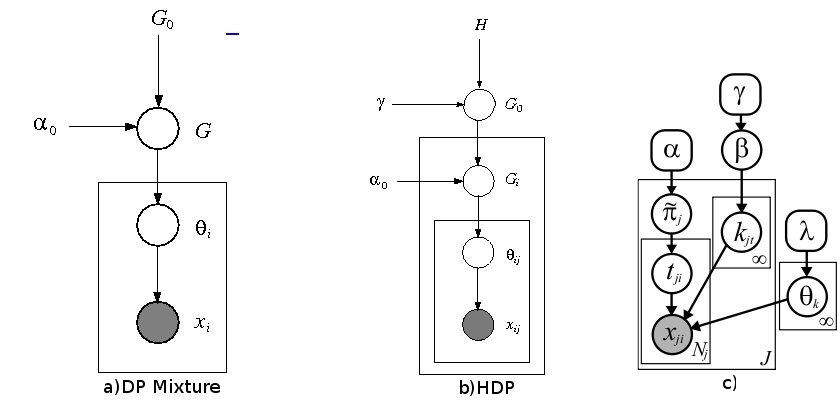
\includegraphics[width=1.0\textwidth]{gm.jpg} 
    \caption{a)b)Graphical Model for DP mixture and HDP.  c)Graphical Model for HDP with CRF construction} 
    \label{fig:by:table} 
\end{figure}


\subsection{ME Algorithm}
Consider a probabilistic model P(x,w,$\alpha$),where x is observed random variable, w hidden variable and $\alpha$ hyperparameter.   
For the generative approach to clustering, hidden variables are divided into two classes: cluster assignment z and generative model parameters $\theta$.  
The typical task is machine learning is to estimate the distribution of hidden variable w: p(w$|\alpha$)=p(z,$\theta|\alpha$).
For variational methods, the goal is to find the estimation q(z,$\theta$) that minimizes the KL divergence from posterior distribution $p(z,\theta |\vec x,\alpha)$, which 
is equivalent to maximizing the lower bound $\mathcal{L}(q(z,\theta))$ for the likelihood:
\begin{eqnarray*}
log p(\vec x |\alpha)
&\geq&\mathcal{L}(q(z,\theta)) \\
&=&log p(\vec x | \alpha)-KL[q(\theta,\vec z) || p(\theta,\vec z | \vec x,\alpha)] \\
&=&-\boldmath{E}[log p(\vec x,\vec z, \theta | \alpha)]_{q(\theta,\vec z)}-H[q(\theta,\vec z)] 
\end{eqnarray*}
where $H(q(w))=-\int_w \ q(w)log [q(w)] dw$ is the entrophy.
Instead of estimating the joint distribution q(z,$\theta$), the normal approach is to factorize it into q(z)q($\theta$) which can be updated iteratively as coordinate ascent. 
In general, we can either maintains distribution estimation(known as E-step) or point estimation(known as M-step) for the hidden variable.
The popular Meanfield method iteratively estimates the disribution for z and $\theta$ with the following formula.
\begin{center}
$q (\theta ) \propto exp(E[log P(\theta, z, D)]_{q(z)} ) \longleftrightarrow q (z) \propto  exp(E[log P(\theta, z, D)]_{q (\theta )})$.
\end{center}
In contrast, K-means algorithm keeps a point estimation for both $\theta$ and z. 
Discussed in [4], we can have four combinations of E-step and M-step for z and $\theta$. 
For our interest, we find ME algorithm(M-step for z, E-step for $\theta$) particularly fit for the clustering problem for the following reasons:\\

1) In pratice, people may just want the optimal solution for the cluster assignment z instead of the real distribution of q(z).
Thus point estimation for z is enough\\

2) For most of the time, the cluster assignment z is discrete and high dimensional, which makes the update formula non-analytic and hard to approximate. \\

So instead of maintaining the huge matrix for q(z), we may just pick out the MAP estimator(M-step) for q(z).
Since we don't want to be too greedy to also take M-step for q($\theta$), we end up with ME algorithm.


\section{ME Algorithm for HDP}  
Since the E-step for $\theta$ is trivial, the key of ME learning algorithm lies in the optimization problem of searching cluster assignment z.
\subsection{Formula}
For Dirichlet Process Mixture Model (DPM) with Gaussian conjugated with Normal-Inverse-Wishart(NIW) distribution, Below is the derivation from [4].\\ \\ 
\emph{Likelihood Term}:$\ \ \ \ \ \ \ \ \ p(x_{n},\theta|\lambda,z_{n})=\mathcal{N}(x_{n}|z_{n},\mu,\Omega)
\mathcal{N}(\mu|m_{0},\xi_{0}\Omega)\mathcal{W}(\Omega|\eta_{0},B_{0})$\\ 
\emph{Assignment Term}: $\ \ \ \ \ \ p(\vec z|\lambda)=\frac{\Gamma(\phi_{0})}{\Gamma(N+\phi_{0})}\Pi_{k=1}^{K}\Gamma(N_{k}) \phi_{0}^{K}$\\
\emph{Object Function}: $\ \ \ \ \ \ \ log(p(x,z|\lambda))=log(p(x|z,\lambda))+log(p(z|\lambda))=$\\
(Likelihood)$ -\frac{D N}{2}log\pi-\sum_{k=1}^{K} [\frac{D}{2}log\frac{\xi_{k}}{\xi_{0}}+\frac{\eta_{k}}{2}log det(B_{k})-\frac{\eta_{0}}{2}log det(B_{0})
-log \frac{\Gamma_{D}(\frac{\eta_{k}}{2})}{\Gamma_{D}(\frac{\eta_{0}}{2})}]$
\\
+
\\
(Assignment:)$log(\frac{\Gamma(\phi_{0})}{\Gamma(N+\phi_{0})})+\sum_{k=1}^{K}[log \Gamma(N_{k})+log\phi_{0}]$\\ 
where:\\
D: dimension of a data point\\ 
N: total number of datas\\ 
$N_{k}$: number of datas in cluster k\\ 
$S_{k}$: the covariance of datas in cluster k\\ 
$\phi_{k}=\phi_{0}+N_{k}$\\
$m_{k}=\frac{N_{k}\bar x_{k}+\xi_{0}m_{0}}{\xi_{k}}$\\
$B_{k}=B_{0}+N_{k}S_{k}+\frac{N_{k}\xi_{0}}{\xi_{k}}(\bar x_{k}-m_{0})(\bar x_{k}-m_{0})^{T}$\\
$\eta_{k}=\eta_{0}+N_{k}$\\
$\xi_{k}=\xi_{0}+N_{k}$\\
$\Gamma_{D}(x)=\pi^{\frac{D(D-1)}{4}}\Pi_{i=1}^{D}\Gamma(x+\frac{1-i}{2})$ \\ \\
For HDP, we only need to change Assignment term. Here we use the Chinese Restaurant Franchise Representation.\\
Notation: J Restaurants, K global dishes, T tables, N datas,\\
$t_{ji}:$ the table that customer i in Restaurant j sits;\\
$k_{jt}:$ the dish that table t in Restaurant j serves;\\
$m_{jk}:$ number of tables in Restaurant j serving dish k;\\
$m_{.k}:$ number of tables serving dish k;\\
$m_{j.}:$ number of tables in Restaurant j;\\
$m_{..}:$ number of tables;\\
$n_{jtk}:$ number of customers in Restaurant j at table t eating dish k;\\
$n_{jt.}:$ number of customers in Restaurant j at table t;\\
$n_{j..}:$ number of customers in Restaurant j;\\
$p(k_{jt}|\vec k_{1},...\vec k_{j-1},k_{j1},...,k_{j(t-1)},\gamma)=\sum_{k=1}^{K}\frac{m_{.k}}{m_{..}-1+\gamma}\delta_{k_{jt}=k}+\frac{\gamma}{m_{..}-1+\gamma}\delta_{k_{ji}=\vec k}$\\ 
$p(t_{ji}|t_{j1},...,t_{j(i-1)},\alpha)=\sum_{t=1}^{m_{j.}}\frac{n_{jt.}}{i-1+\alpha}\delta_{t_{ji}=t}+\frac{\alpha}{i-1+\alpha}\delta_{t_{ji}=\vec t}$\\ 
$p(\vec z|\lambda)=p(\vec t,\vec k|\lambda)=\Pi_{j=1}^{J}[\frac{\Gamma(\alpha)}{\Gamma(n_{j..}+\alpha)}\Pi_{t=1}^{m_{j.}}(\Gamma(n_{jt.}))]\alpha^{\sum_{j=1}^{J}m_{j.}}
\times \frac{\Gamma(\gamma)}{\Gamma(T+\gamma)}\Pi_{k=1}^{K} [\Gamma(m_{.k})] \gamma^{K}$ \\ \\
So the goal of ME algorithm is to search for the assignment variable $\vec t,\vec k$ that maximizes
$log(p(x,z|\lambda))$=\\
(Likelihood)$-\frac{D n_{...}}{2}log\pi-\sum_{k=1}^{K} [\frac{D}{2}log\frac{\xi_{k}}{\xi_{0}}+\frac{\eta_{k}}{2}log det(B_{k})-\frac{\eta_{0}}{2}log det(B_{0})
-log \frac{\Gamma_{D}(\frac{\eta_{k}}{2})}{\Gamma_{D}(\frac{\eta_{0}}{2})}]$ \\ 
+\\
(Assignment:)$\sum_{j=1}^{J}\{log \frac{\Gamma(\alpha)}{\Gamma(n_{j..}+\alpha)}+\sum_{t=1}^{m_{j.}}[log(\Gamma(n_{jt.})+log \alpha]\}+
 log \frac{\Gamma(\gamma)}{\Gamma(T+\gamma)}+\sum_{k=1}^{K} [log(\Gamma(m_{.k})+log \gamma]$\\ \\

\subsection{Pseudocode}
We first try local search methods, corresponding to Posterior Gibbs Sampling in [7] and then add split\&merge approach. We randomized the algorithm
by randomly permute the order during searching.Detailed Pseudocode can be seen in the Appendix.\\

{\bf Pseudocode:}\\
b$\sim$Uniform[0,1]\\
Switch (ceil(b*6)):\\
case 1: Local Search the best table for each customer\\
case 2: Local Search the best dish for each table\\
case 3: Split each table in each restaurant\\
case 4: Split each dish\\
case 5: Merge tables in each restaurant\\ 
case 6: Merge dishes\\
\section{Results for Synthetic Data}
\subsection{Dirichlet Process Mixture}
We test Meanfield algorithm (EE) [1], Collapsed Meanfield algorithm(Collapsed EE)[5] and ME algorithm [3] implemented by Kurihara on the synthetic data, 200 random samples drawn from Gaussian of four mixtures.
We set the same hyperparameters for these three algorithms and test with different initial cluster numbers.
Results are summarized in table 1. 
From figure 2 c),d), we can see that to some degree both EE and Collapsed EE suffer from local minimas and do not have other ways out.
Three variants of ME algorithms are tested here. The hierarchical clustering methods--bottom up and top down-- work perfect on the synthetic data and 
a naive local search+ merge works reasonably well.
The advantage of ME algorithm is that it can be easily extended with advanced search methods to escape local minima.
\begin{figure}[h] 
    \centering 
    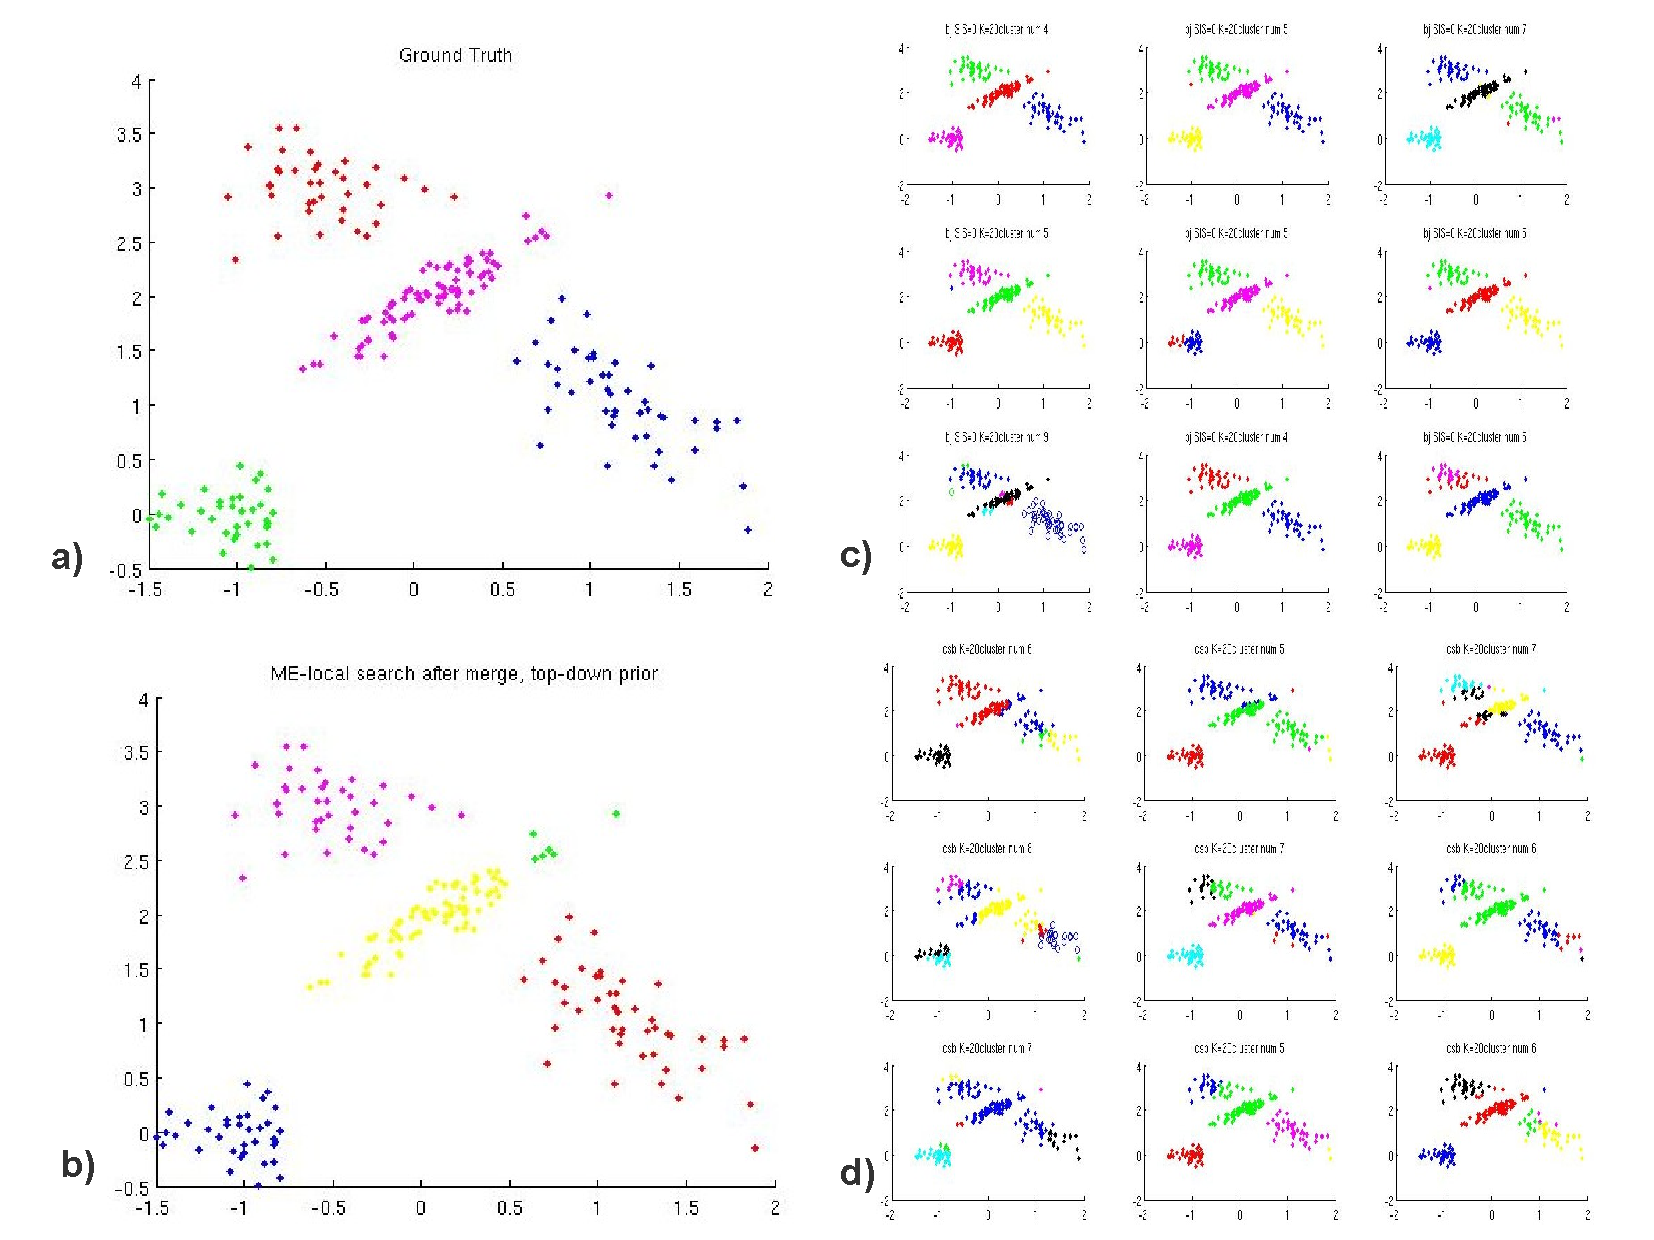
\includegraphics[width=1.0\textwidth]{me_dp.pdf} 
    \caption{a)Ground Truth. b)One run of local search+merge.c)Nine runs for EE.c)Nine runs for Collapsed EE} 
    \label{fig:by:table} 
\end{figure}



\begin{table}[t]
\caption{Comparison of EE, Collapsed-EE and ME algorithms for DP mixture(with mean and std)}
\begin{center}
\begin{tabular}{|l|l|l|l|}

\hline
{\bf Learning Algorithm} &{\bf Initial Cluster Numbers} &{\bf Number of clusters}  &{\bf RandIndex} \\ 
\hline 
\multirow{2}{*}{EE(sampled initialization)} & 10 & 4.1(0.3) & 0.99(0.00) \\
					    & 20 & 4.1(0.3) & 0.99(0.00)\\
\hline
\multirow{2}{*}{EE(random initialization)}  & 10 & 6.9(1.2)&  0.97(0.01) \\
					    & 20 & 7.6(1.7)&  0.93(0.02) \\
\hline
\multirow{2}{*}{Collapsed EE}               & 10 & 5.6(1.6)&  0.90(0.22) \\
					    & 20 & 7.4(0.9)&  0.87(0.09) \\
\hline
\multirow{4}{*}{ME}                         & 1(Top-down) &    4  &  1 \\
					    & 200(Bottom-up) & 4  &  1 \\
					    & 200(Local search) & 15.5(3.9)&  0.83(0.09) \\
					    & 200(Local search+Merge) & 6.5(0.9)&  0.93(0.09) \\
\hline
\end{tabular}
\end{center}
\end{table}
\subsection{Hierarchical Dirichlet Process}
{\bf Synthetic data:}\\
 9 restaurants, each of which has 200 customers drawn from a mixture of 14 2-d Gaussian distributions.\\
{\bf Interpretation:}\\
From Figure 3 a), we can see that dishes with the same color are shared among restaurants, which simulates the expected situation that topics are shared among documents.\\
From Figure 3 c), Local search algorithm gets stuck at a local maxima where tables tend to be big.e.g. For the restaurant in the center, it should be 
splitted into 5 dishes instead of 3.\\
From Figure 3 d), the bad configuration mentioned above is avoided by using bigger search moves: split and merge, which is almost the same to the ground truth.\\
From Figure 3 b), there are nine blue lines representing 9 runs of Local Search, where the end points diverge. But after split and merge, 
the log probability converges to a better local maxima. 
\begin{figure}[h] 
    \centering 
    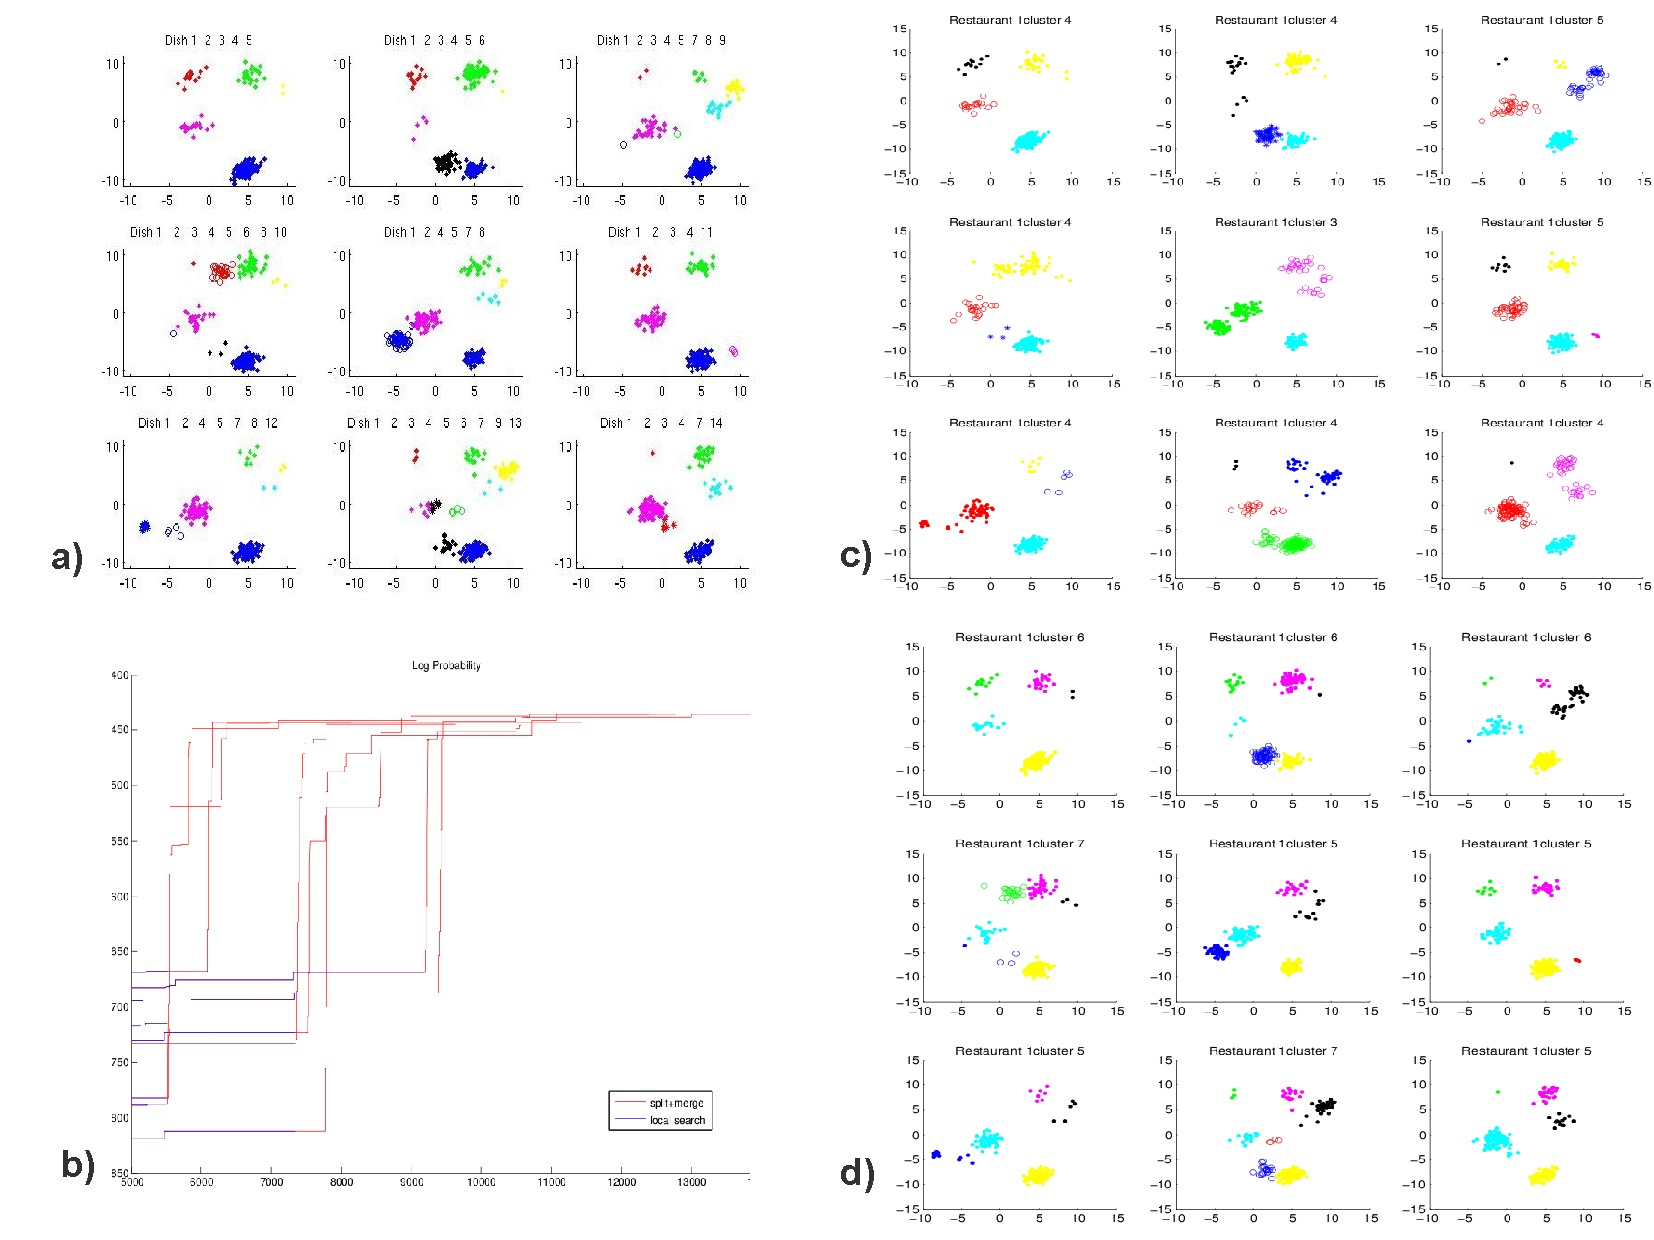
\includegraphics[width=1.0\textwidth]{me_hdp.pdf} 
    \caption{a)Ground Truth for  for DP mixture and HDP.  c)Graphical Model for HDP with CRF construction} 
    \label{fig:by:table} 
\end{figure}
\section{Conclusion}
In this report, we first show the advantage of ME alogorithm over other variational methods to learn Dirichlet Process Mixture Model. Later we 
develop the randomized ME algorithm for Hierarchical Dirichlet Process Model, which works reasonably well on the toy data. Our future 
direction is to improve and test the algorithm on real data sets for document classification and natural image segmentation.c


\section{References}
\small{
[1]  Blei,D,M, Jordan,M.I, and Ng, A. Y. (2003), “Hierarchical Bayesian Models for Applications 
  in Information Retrieval,” in Bayesian Statistics, vol. 7, pp. 25–44 

[2] E.B.Sudderth and M.I.Jordan(2008)Shared Segmentation of Natural Scenes Using Dependent Pitman-Yor Processes NIPS 2008


[3] Ghahramani, Z. and Beal, M. J. (2000). Variational inference for Bayesian mixtures of                                                          ̈
  factor analysers. In S. A. Solla, T. K. Leen, \& K.-R. Muller (Eds.), Advances in neural
  information processing systems, 12. Cambridge, MA: MIT Press.

[4] K. Kurihara and M. Welling. Bayesian K-means as a
 ”maximization-expectation” algorithm. Neural Computation, 2008

[5] Y. W. Teh, K. Kurihara and M. Welling. Collapsed Variational Inference for HDP
NIPS 2007

[6] Y. W. Teh and M.I.Jordan.Hierarchical Bayesian Nonparametric Models with Applications.(2010) Bayesian 
Nonparametrics in Practice, Cambridge, UK: Cambridge University Press.

[7] Y. W. Teh, M. I. Jordan, M. J. Beal, and D. M. Blei. Hierarchical Dirichlet processes. Journal of the 
American Statistical Association, 101(476):1566–1581, 2006.

[8] Hal Daume ́III Fast search for Dirichlet process mixture models. UAI 2006
}
\section{Appendix}
\subsection{Pseudocode of ME algorithm for HDP}

\begin{enumerate}
\item Split tables:\\
0) Randomly pick a Restaurant R with m tables.\\
   Randomly pick the a table with n customers.\\ 
1) if(n$\neq$1) Do 2-means++ 
\begin{enumerate}
\item First 2 points:\\ \\
Randomly pick a customer C1 from table T to form a new table (m+1)\\
Randomly sample a dish(can be new) for the new table (m+1) according to the cost\\
Randomly sample another customer C2 from table t according to the cost\\
Randomly sample a dish(can be new) for the new table (m+2) according to the cost\\ \\
\item Initialization:\\ \\
For ww=randperm(customers from table T except C1,C2) \\ 
Randomly sample the table assignment zz$\in \{m+1,m+2\}$ for customer ww according to the cost\\
Randomly sample a dish(can be new) for table zz according to the cost\\
End \\ \\
\item Iteration(2-means):\\ \\
While no more changes of table config and dish config can increase P:\\
b=rand([0,1]) \\
Switch (ceil(b*4)):\\
case 1: Randomly pick a customer from table (m+1), assign it to table (m+2) if the change increase P\\
case 2: Randomly pick a customer from table (m+2), assign it to table (m+1) if the change increase P\\
case 3: pick table (m+1), assign it the dish which increase P mostly\\
case 4: pick table (m+2), assign it the dish which increase P mostly\\
End\\
\end{enumerate}  

\item Merge table:\\
0) Randomly pick a Restaurant R, which has m tables.\\
1) Interation:\\
 While no more changes of table assignment and dish assignment can increase P:\\
 b=rand([0,1]) \\
 Switch (ceil(b*2)):\\
 case 1: Randomly pick a table in R, merge it to the table in R which increase P mostly\\
 case 2: Randomly pick a table in R, assign it the dish which increase P mostly\\
 End\\


\item Split dishes:\\
0) Randomly pick a Restaurant dish k, which has m tables.\\
1) if(m$\neq$1) Do 2-means++ (current: K dishes,dish assignment:$z_{k0}$)\\
\begin{enumerate}
\item First 2 tables:\\
Randomly pick a table t1 in from dish k.\\
Randomly sample a dish k1 for table t1 according to the cost \\
Randomly sample another table t2 from dish k according to weight\\
Randomly sample a dish k2 for table t2 according to the cost 
\item Initialization:\\
For ww=randperm(tables from dish k except t1,t2) \\ 
Randomly sample a dish assignment zz$\in\{k1,k2\}$ for table ww\\
End 
\item Iteration(2-means):\\ \\
While no more changes of dish assignment can increase P:\\
b=rand([0,1]) \\
Switch (ceil(b*2)):\\
case 1: Randomly pick a table from dish k1, assign it to dish k2 if the change increase P\\
case 2: Randomly pick a table from dish k2, assign it to dish k1 if the change increase P\\
End
\end{enumerate}  

\item Merge dishes:\\
1) if(K$\neq$1) Do: \\ \\
 While no more changes of dish assignment can increase P:\\
 Randomly pick a dish, merge it to the dish which increase P mostly\\
 End\\
\end{enumerate}  


\end{document}
